\documentclass{beamer}
\usetheme{Madrid}
\usepackage[utf8]{inputenc}
\usepackage{physics}
\usepackage{csquotes}
\def\signed #1{{\leavevmode\unskip\nobreak\hfil\penalty50\hskip1em
  \hbox{}\nobreak\hfill #1%
  \parfillskip=0pt \finalhyphendemerits=0 \endgraf}}

\newsavebox\mybox
\newenvironment{aquote}[1]
  {\savebox\mybox{#1}\begin{quote}\openautoquote\hspace*{-.7ex}}
  {\unskip\closeautoquote\vspace*{1mm}\signed{\usebox\mybox}\end{quote}}

\usepackage{qcircuit}

\usepackage{tikz}
\usetikzlibrary{arrows,shapes}
\newcommand{\tikzmark}[1]{\tikz[remember picture] \node[coordinate] (#1) {#1};}
\tikzstyle{block} = [rectangle, draw, text centered, minimum width = 2em, minimum height=4em]
\tikzstyle{redblock} = [rectangle, draw, fill=red!20, text centered, minimum width = 2em, minimum height=4em]

%Information to be included in the title page:
\title{Quantum Error Correction}
\author[GGHLZ]{Louis Golowich \and Wenjie Gong \and Ari Hatzimemos\\ Dylan Li \and Dylan Zhou}
\institute[Harvard University]{Physics 160 \\ Harvard University}
\date[Physics 160 Final Project]{Final Project Presentation, 13 May 2020}

\begin{document}

\frame{\titlepage}

\begin{frame}
    \frametitle{Table of Contents}
    \tableofcontents
\end{frame}

\section{Introduction and Review of Quantum Error Correction}
\begin{frame}
\frametitle{Introduction}
    \begin{aquote}{William Blake}
        To be an Error and to be Cast out is part of God's Design.
    \end{aquote}
    \vspace{15mm}
    \begin{itemize}
        \item Noise as a longstanding problem in information processing systems
            \begin{itemize}
                \item \textit{e.g.}, classical computers, modems, CD players, etc.
                \item  Noise is still a problem in quantum information
            \end{itemize}
        \item Key idea: to protect a message against noise, \textit{encode} the message by adding redundant information; even if some information is corrupted, redundancy allows us to \textit{decode} and recover the original message
    \end{itemize}
\end{frame}

\begin{frame}
    \frametitle{Project Framework}
    \begin{itemize}
        \item Goals: 
        \begin{itemize}
            \item to implement various quantum error-correcting codes
            \begin{itemize}
                \item we chose the 3-qubit, 9-qubit, 7-qubit codes
            \end{itemize}
            \item to analyze and compare their performances 
            \begin{itemize}
                \item \textit{when are they effective?}
                \item \textit{when should we use error-correcting codes?}
            \end{itemize} 
        \end{itemize}
        \item Tools:
        \begin{itemize}
            \item Python's Qiskit package
            \item IBM's quantum machines
        \end{itemize}
    \end{itemize}
\end{frame}

\section{The 3-Qubit Codes}
\begin{frame}
    \frametitle{3-Qubit Codes: Classical Inspiration}
    \textbf{Classical Error Correction}
    \begin{itemize}
        \item Encoding by \textit{repetition codes}:
        \begin{align*}
            &0 \rightarrow 000 \\
            &1 \rightarrow 111.
        \end{align*}
        \item Decoding by \textit{majority voting}:
        \begin{align*}
            \textit{Ex.: }\,\, 001 \rightarrow 0.
        \end{align*}
        \item Analysis: Let $p$ be the probability that a bit is flipped. This method fails when 2 or more bits are flipped, which occurs with probability $3p^2(1-p)+p^3$, so the probability of error is $p_e = 3p^2-2p^3$. Then this method is preferred when $p_e < p$, or $p < 1/2$.
    \end{itemize}
\end{frame}

\begin{frame}
    \frametitle{Noisy Channels: The Bit Flip Channel}
    %\textbf{The Quantum Version: 3-Qubit Bit Flip Code}
    \begin{itemize}
        \item One model for noise is the \textit{bit flip channel} (analogous to classical channel).
        \item The bit flip channel flips qubits with probability $p$ and leaves them untouched with probability $1-p$.
        \item Equivalent to applying $X$ gate with probability $p$.
        \item We protect qubits from this channel with the \textit{bit flip code}.

    \end{itemize}
\end{frame}

\begin{frame}
    \frametitle{3-Qubit Bit Flip Code: Encoding Logical Bits}
    %\textbf{The Quantum Version: 3-Qubit Bit Flip Code}
    \begin{itemize}
        \item The goal is to correct bit flip errors.
        \item Encoding:
        \begin{align*}
            &\ket{0} \rightarrow \ket{0_L} \equiv \ket{000} \\
            &\ket{1} \rightarrow \ket{1_L} \equiv \ket{111}.
        \end{align*}
        \item Encoding circuit for 3-qubit bit flip code:
    
        \vspace{5mm}
        \hspace{48mm}
        \Qcircuit @C=1em @R=1.5em {
        \lstick{\ket{\psi}} & \ctrl{1} & \ctrl{2} & \qw \\ 
        \lstick{\ket{0}} & \targ & \qw & \qw \\
        \lstick{\ket{0}} & \qw & \targ & \qw
        }

    \end{itemize}
\end{frame}

\begin{frame}
    \frametitle{3-Qubit Bit Flip Code: Detecting Errors}
    %\textbf{3-Qubit Bit Flip Code: Detecting Errors}
    \begin{itemize}
        \item Suppose there is a bit flip error after encoding:
    
        \vspace{5mm}
        \hspace{37mm}
        \Qcircuit @C=1em @R=1.5em {
        \lstick{\ket{\psi}} & \ctrl{1} & \ctrl{2} & \qw & \multigate{2}{E_{\text{bit}}} & \qw\\ 
        \lstick{\ket{0}} & \targ & \qw & \qw & \ghost{E_{\text{bit}}} & \qw\\
        \lstick{\ket{0}} & \qw & \targ & \qw & \ghost{E_{\text{bit}}} & \qw
        }\vspace{5mm}

        \item Error Detection (or \textit{syndrome diagnosis}):
            \begin{itemize}
                \item we would like to determine which, if any, of the qubits have been corrupted
                \item four error syndromes: no error, bit flip on qubit one, bit flip on qubit two, bit flip on qubit three
            \end{itemize}

    \end{itemize}
\end{frame}

\begin{frame}
    \frametitle{3-Qubit Bit Flip Code: Detecting Errors}
    % \textbf{The Quantum Version: 3-Qubit Bit Flip Code}
            \begin{itemize}
                \item We can diagnose the syndrome using two ancillary qubits:
                
            \vspace{5mm}
            \hspace{10mm}
            \Qcircuit @C=1em @R=1.5em {
            \lstick{\ket{\psi}} & \ctrl{1} & \ctrl{2} & \qw & \multigate{2}{E_{\text{bit}}} & \qw & \ctrl{3} & \qw & \ctrl{4} &\qw &\qw\\ 
            \lstick{\ket{0}} & \targ & \qw & \qw & \ghost{E_{\text{bit}}} & \qw & \qw & \ctrl{2} & \qw & \qw\ & \qw\\
            \lstick{\ket{0}} & \qw & \targ & \qw & \ghost{E_{\text{bit}}} & \qw &  \qw & \qw & \qw & \ctrl{2} & \qw\\
            & & & &  &\lstick{\ket{0}} & \targ & \targ & \qw & \qw  & \qw & \meter\\
            & & & &  &\lstick{\ket{0}} & \qw & \qw & \targ & \targ & \qw &\meter
            } \vspace{5mm}

            \item Based on measurement results, we know where the error occured.
            \end{itemize}

\end{frame}

\begin{frame}
    \frametitle{3-Qubit Bit Flip Code: Correcting Errors}
    % \textbf{3-Qubit Bit Flip Code: Correcting Errors}
    \begin{itemize}
        \item Complete circuit for error correction (or \textit{recovery}):
        
            \vspace{5mm}
            \includegraphics[scale=0.35]{3qb-circuit.png}
    \end{itemize}
\end{frame}

\begin{frame}
    \frametitle{Analyzing the Bit Flip Code: Simulation}
    % \textbf{3-Qubit Bit Flip Code: Correcting Errors}
    \begin{itemize}
        \item<1-> Let's look at the performance of the 3-qubit bit flip code against bit flip channels of varying error probabilities $p$.
        \item<2-> Setup: 
        \begin{enumerate}
            \item encode a single qubit in state $\ket{0}$ into a logical state $\ket{0_L} = \ket{000}$
            \item create a bit flip channel which adds $X$ gates with probability $p$
            \item run error correcting code
            \item measure final state 
        \end{enumerate}
        \item<3-> We can calculate the accuracy of the error correcting code for a given $p$ by repeating many times and taking the number of times we measure a correct final state $\ket{000}$ and dividing by the total number of trials.
        \item<4-> We can compare this to the accuracy of a single qubit (without encoding or error correction) that goes through a bit flip channel with the same $p$ to see when error correction is effective.
    \end{itemize}
\end{frame}

\begin{frame}
    \frametitle{Analyzing the Bit Flip Code: Simulation}
    % \textbf{3-Qubit Bit Flip Code: Correcting Errors}
    \begin{itemize}
        \item Ran tests on Qiskit's simulator
        \item Probability $p$ ranging from 0 to 1; 10000 trials for each $p$
    \end{itemize}
    \begin{minipage}{0.45\textwidth}
        \begin{figure}[H]
        \includegraphics[scale=0.4]{3qb-bf-overlay copy.png}
        % \caption{\label{fig:blue_rectangle} Rectangle}
        \end{figure}
        \end{minipage} \hfill
        \begin{minipage}{0.45\textwidth}
        \begin{itemize}
        \item Observe crossover point at $p=0.5$.
        \item For $p<0.5$, error correcting code performs better than a single qubit with no correction.
        \end{itemize}
    \end{minipage}
\end{frame}



\begin{frame}
    \frametitle{Noisy Channels: Phase Flip Channel}
    % \textbf{3-Qubit Bit Flip Code: Correcting Errors}
    \begin{itemize}
        \item Another quantum channel is the \textit{phase flip} error model.
        \item With probability $p$ the relative phase of states $\ket{0}$ and $\ket{1}$ is flipped, with probability $1-p$ it is left alone.
        \item Equivalent to applying $Z$ operator with probability $p$.
        \item We fight this channel with the \textit{phase flip code}.
    \end{itemize}
\end{frame}

\begin{frame}
    \frametitle{3-Qubit Phase Flip Code}
    % \textbf{3-Qubit Bit Flip Code: Correcting Errors}
    \begin{itemize}
        \item No classical analog, but it is easy to turn the phase flip channel into a bit flip channel.
        \item Use $x$-basis for encoding:
        \begin{align*}
            &\ket{0} \rightarrow \ket{0_L} \equiv \ket{+++} \\
            &\ket{1} \rightarrow \ket{1_L} \equiv \ket{---}.
        \end{align*}    
        \item Phase flip $Z$ acts as bit flip for this encoding!

    \end{itemize}
\end{frame}

\section{The Shor 9-Qubit Code}
\begin{frame}
    \frametitle{The Shor Code}
    \begin{itemize}
        \item<1-> Can we protect against \textit{arbitrary} errors?
        \item<2-> Yes! $\longrightarrow$ The \textit{Shor code}
    \end{itemize}
\end{frame}

\begin{frame}
    \frametitle{The Shor Code: Encoding}
    \begin{itemize}
        \item By combining the 3-qubit phase flip and bit flip codes, the Shor code protects against arbitrary errors.
        \item First encode the qubit using the phase flip code: $$\ket{0}\rightarrow\ket{+++},\quad \ket{1}\rightarrow\ket{---}.$$
        \item Then encode each of those qubits with the bit flip code: $$\ket{+}\rightarrow (\ket{000}+\ket{111})/\sqrt{2},\quad \ket{-}\rightarrow (\ket{000}-\ket{111})/\sqrt{2.}$$
        \item The result is a 9-qubit code with codewords 
        \begin{align*}
            & \ket{0} \rightarrow \ket{0_L} \equiv \frac{(\ket{000} + \ket{111})(\ket{000} + \ket{111})(\ket{000} + \ket{111})}{2\sqrt{2}}\\
            & \ket{1}\rightarrow \ket{1_L} \equiv \frac{(\ket{000} - \ket{111})(\ket{000} - \ket{111})(\ket{000} - \ket{111})}{2\sqrt{2}}.
        \end{align*}
    \end{itemize}
\end{frame}

% \begin{frame}
%     \frametitle{The Shor 9-Qubit Code: A Review}
%     \textbf{Encoding}
%         \begin{itemize}
%         \item The goal is to correct an arbitrary single bit error and/or phase error on any of the nine physical qubits.
%         \item The 9-qubit code encodes a single state into a logical state of nine physical qubits, arranged in blocks of three.
%         \item Encoding:
    
%         \begin{align*}
%             &\ket{0} \rightarrow \ket{0_L} \equiv \frac{1}{\sqrt{8}}(\ket{000}+\ket{111})(\ket{000}+\ket{111})(\ket{000}+\ket{111}) \\
%             &\ket{1} \rightarrow \ket{1_L} \equiv \frac{1}{\sqrt{8}}(\ket{000}-\ket{111})(\ket{000}-\ket{111})(\ket{000}-\ket{111}).
%         \end{align*}

%     \end{itemize}
% \end{frame}

\begin{frame}
    \frametitle{The Shor 9-Qubit Code: Encoding}
        Encoding circuit for 9-qubit code:
        
        \begin{center}
        \includegraphics[scale=0.7]{9qbencoding.PNG}
        \end{center}
\end{frame}

\begin{frame}
    \frametitle{The Shor 9-Qubit Code: Correcting Errors}
    \textbf{Bit Flip Error Correction}
        \begin{itemize}
            \item On each block of three (i.e. qubits 0-2, 3-5, and 6-8), the 3-qubit circuit is utilized to correct for bit flips.
        \end{itemize}
        \textbf{Phase Flip Error Correction}
        \begin{itemize}
            \item The phase of the first two blocks of three (qubits 0-2 and 3-5) and the second two blocks of three (qubits 3-5 and 6-8) are compared to correct for phase flips.
            \item The phase correction necessitates two ancillary qubits. Thus, we need 8 ancilla: 6 for bit flip correction, and 2 for phase flip correction.
        \end{itemize}
\end{frame}

\begin{frame}
    \frametitle{The Shor 9-Qubit Code: Correcting Phase Errors}
        \begin{itemize}
            \item The phase correction circuit, shown below, converts the qubits from the x-basis to the z-basis and checks parity of each block of two.
            \begin{center}
            \includegraphics[scale=0.5]{9qbphase.PNG}
            \end{center}
        \end{itemize}
\end{frame}


\begin{frame}
    \frametitle{The Shor 9-Qubit Code: Correcting Phase Errors}
        \begin{itemize}
            \item The following corrections are performed depending on the measured ancilla for phase flip correction:
            
            \begin{align*}
            &10 \rightarrow \sigma_z \text{ on block 1}\\
            &01 \rightarrow \sigma_z \text{ on block 2}\\
            &11 \rightarrow \sigma_z \text{ on blocks 1 and 2}.\\
           \end{align*}
        
            
        \end{itemize}
\end{frame}

\begin{frame}
    \frametitle{The Shor 9-Qubit Code: Error Correction Methodology}
        \begin{itemize}
            \item We only consider error that occurs between the encoding step and the correcting step, thus simulating a memory error.
            \begin{center}
                \includegraphics[scale = 0.08]{9qberror.png}
            \end{center}
            \item Specifically, we consider a complete phase flip and/or bit flip (i.e. $X$ or $Z$) that occurs independently on each of the 9 physical qubits with probability $p$.
            \item After the error, we measure the ancilla and apply the appropriate error correcting steps. Finally, we run the encoding circuit in reverse and measure the output to determine fidelity.
        \end{itemize}
\end{frame}

\begin{frame}
    \frametitle{The Shor 9-Qubit Code: Simulation Performance with No Error Correction}
        \begin{itemize}
            \item Initial state: $\ket{0} \rightarrow \ket{0_L} \equiv \frac{1}{\sqrt{8}}(\ket{000}+\ket{111})(\ket{000}+\ket{111})(\ket{000}+\ket{111})$.
            \item Fidelity of un-encoded state measured against $\ket{000000000}$.
            
            \centering\includegraphics[scale = 0.5]{shor9_nec.pdf}
        \end{itemize}
\end{frame}

\begin{frame}
    \frametitle{The Shor 9-Qubit Code: Simulation Performance with Error Correction}
            \centering\includegraphics[scale = 0.7]{shor9_ec.pdf}
\end{frame}

\section{The 7-Qubit Code}
\begin{frame}
  \frametitle{7-Qubit Code}
  Encodes 1 logical qubit using 7 physical qubits:
  {\tiny
    \begin{align*}
      \ket{\overline{0}} &= \frac{\ket{0000000}+\ket{1010101}+\ket{0110011}+\ket{1100110}+\ket{0001111}+\ket{1011010}+\ket{0111100}+\ket{1101001}}{\sqrt{8}} \\
      \ket{\overline{1}} &= \frac{\ket{1111111}+\ket{0101010}+\ket{1001100}+\ket{0011001}+\ket{1110000}+\ket{0100101}+\ket{1000011}+\ket{0010110}}{\sqrt{8}}
    \end{align*}
    \begin{align*}
      H^{\otimes 7}\ket{\overline{0}} &= \frac{\ket{\overline{0}}+\ket{\overline{1}}}{\sqrt{2}} \\
      H^{\otimes 7}\ket{\overline{1}} &= \frac{\ket{\overline{0}}-\ket{\overline{1}}}{\sqrt{2}}
    \end{align*}
  }
\end{frame}

\begin{frame}
  \frametitle{7-Qubit Code}
  \vspace{-1cm}
  {\tiny
    \begin{align*}
      \ket{\overline{0}} &= \frac{\ket{0000000}+\ket{1010101}+\ket{0110011}+\ket{1100110}+\ket{0001111}+\ket{1011010}+\ket{0111100}+\ket{1101001}}{\sqrt{8}} \\
      \ket{\overline{1}} &= \frac{\ket{1111111}+\ket{0101010}+\ket{1001100}+\ket{0011001}+\ket{1110000}+\ket{0100101}+\ket{1000011}+\ket{0010110}}{\sqrt{8}}
    \end{align*}
    \begin{align*}
      H^{\otimes 7}\ket{\overline{0}} &= \frac{\ket{\overline{0}}+\ket{\overline{1}}}{\sqrt{2}} \\
      H^{\otimes 7}\ket{\overline{1}} &= \frac{\ket{\overline{0}}-\ket{\overline{1}}}{\sqrt{2}}
    \end{align*}
  }
  \begin{itemize}
  \item Of the 16 bit strings above, any two differ by $\geq 3$ bits
  \item Intuition: therefore a single bit flip can be recovered
    \begin{itemize}
    \item $X$ error flips bit in $\ket{\overline{0}},\ket{\overline{1}}$
    \item $Z$ error flips bit in $H^{\otimes 7}\ket{\overline{0}},H^{\otimes 7}\ket{\overline{1}}$
    \end{itemize}
  \end{itemize}
\end{frame}

% \begin{frame}{7-Qubit Code: Intuition}
%   Example: single bit flip on $1010101$ gives $1011101$
%   \begin{center}
%     \begin{tabular}{ccc}
%       & Bit string & Number bits that disagree \\
%       \hline
%       Want to decode: & 1011101 & \\
%       \hline
%       & 101\textcolor{red}{0}101 & 1 \\
%       & \textcolor{red}{0}0\textcolor{red}{0}\textcolor{red}{0}\textcolor{red}{0}0\textcolor{red}{0} & 5 \\
%     \end{tabular}
%   \end{center}
% \end{frame}

\begin{frame}{Example recovery for $X$ error in qubit 3}
  
  {\tiny
    \begin{align*}
      \ket{\overline{0}} &= \frac{\ket{0000000}+\ket{1010101}+\ket{0110011}+\ket{1100110}+\ket{0001111}+\ket{1011010}+\ket{0111100}+\ket{1101001}}{\sqrt{8}} \\
      X^{(3)}\ket{\overline{0}} &=
                                  \frac{\ket{00\textcolor{red}{1}0000}\tikzmark{t1}
                                  +\ket{10\textcolor{red}{0}0101}\tikzmark{t2}
                                  +\ket{01\textcolor{red}{0}0011}\tikzmark{t3}
                                  +\ket{11\textcolor{red}{1}0110}\tikzmark{t4}
                                  +\ket{00\textcolor{red}{1}1111}\tikzmark{t5}
                                  +\ket{10\textcolor{red}{0}1010}\tikzmark{t6}
                                  +\ket{01\textcolor{red}{0}1100}\tikzmark{t7}
                                  +\ket{11\textcolor{red}{1}1001}\tikzmark{t8}
                                  }{\sqrt{8}}
    \end{align*}

    \begin{equation*}
      \begin{pmatrix}
        1&0&1&0&1&0&1\\
        0&1&1&0&0&1&1\\
        0&0&0&1&1&1&1
      \end{pmatrix}
      \begin{pmatrix}\;\;\\ \\ \tikzmark{n1} \\ \\ \\ \\\end{pmatrix}
      = \begin{pmatrix}1\\1\\0\end{pmatrix} = \ket{3} \text{ (in binary)}
    \end{equation*}
  }
  \begin{tikzpicture}[remember picture,overlay]   %% use here too
    \path[draw=blue,thick,->]<3-> ([xshift=-5mm,yshift=-1mm]t1) -- ([xshift=-2mm,yshift=0mm]n1);
    \path[draw=blue,thick,->]<3-> ([xshift=-5mm,yshift=-1mm]t2) -- ([xshift=-2mm,yshift=1mm]n1);
    \path[draw=blue,thick,->]<3-> ([xshift=-5mm,yshift=-1mm]t3) -- ([xshift=-1mm,yshift=2mm]n1);
    \path[draw=blue,thick,->]<3-> ([xshift=-5mm,yshift=-1mm]t4) -- ([xshift=-1mm,yshift=3mm]n1);
    \path[draw=blue,thick,->]<3-> ([xshift=-5mm,yshift=-1mm]t5) -- ([xshift=1mm,yshift=3mm]n1);
    \path[draw=blue,thick,->]<3-> ([xshift=-5mm,yshift=-1mm]t6) -- ([xshift=1mm,yshift=2mm]n1);
    \path[draw=blue,thick,->]<3-> ([xshift=-5mm,yshift=-1mm]t7) -- ([xshift=2mm,yshift=1mm]n1);
    \path[draw=blue,thick,->]<3-> ([xshift=-5mm,yshift=-1mm]t8) -- ([xshift=2mm,yshift=0mm]n1);
  \end{tikzpicture}
\end{frame}

\begin{frame}{Example recovery for $X$ error}
  \begin{itemize}
  \item In fact:
    \begin{align*}
      \begin{pmatrix}
        1&0&1&0&1&0&1\\
        0&1&1&0&0&1&1\\
        0&0&0&1&1&1&1
      \end{pmatrix}
                     X^{(i)}\ket{\overline{0}} &= \ket{i} \text{ (in binary) for all } i=1,\dots,7
    \end{align*}
  \item Let $H$ be matrix above. To recover from single $X$ error, apply map
    \begin{equation*}
      \ket{v}\otimes\ket{0}_A\mapsto\ket{v}\otimes\ket{Hv}_A
    \end{equation*}
    and measure subsystem $A$. Result will be index $i$ of bit flip, in binary!
  \item Also works for logical state $1$, and for phase flips.
  \end{itemize}
\end{frame}

\begin{frame}{7-qubit code: Why does it work?}
  \begin{itemize}
  \item The kernel of the matrix
    \begin{equation*}
      H=\begin{pmatrix}
        1&0&1&0&1&0&1\\
        0&1&1&0&0&1&1\\
        0&0&0&1&1&1&1
      \end{pmatrix}\in\mathbb{F}_2^{3\times 7}
    \end{equation*}
    consists of the 16 bit strings defining $\ket{\overline{0}},\ket{\overline{1}}$
  \item A bit flip at position $i$ of a vector $v$ adds the $i$th row of $H$ to $Hv$ (basic linear algebra)
  \item The $i$th row of $H$ is $i$ in binary
  \item Same reasoning for phase flips = bit flips in rotated basis
  \end{itemize}
\end{frame}

\begin{frame}{7-qubit code: Initialization}
  
  {\tiny
    \begin{align*}
      \ket{\overline{0}} &= \frac{\ket{0000000}+\ket{1010101}+\ket{0110011}+\ket{1100110}+\ket{0001111}+\ket{1011010}+\ket{0111100}+\ket{1101001}}{\sqrt{8}} \\
      \ket{\overline{1}} &= \frac{\ket{1111111}+\ket{0101010}+\ket{1001100}+\ket{0011001}+\ket{1110000}+\ket{0100101}+\ket{1000011}+\ket{0010110}}{\sqrt{8}}
    \end{align*}
  }
  \begin{center}
    \begin{columns}
      \begin{column}{.1\textwidth}
        \vspace{.15cm}
        \begin{tabular}{c}
          $\ket{\psi}\rightarrow$ \\
          $\ket{0}\rightarrow$ \\
          $\ket{0}\rightarrow$ \\
          $\ket{0}\rightarrow$ \\
          $\ket{0}\rightarrow$ \\
          $\ket{0}\rightarrow$ \\
          $\ket{0}\rightarrow$ \\
        \end{tabular}
      \end{column}
      \hspace{-1cm}
      \begin{column}{.8\textwidth}
        \includegraphics[width=\textwidth]{7qb_init}
      \end{column}
    \end{columns}
  \end{center}
\end{frame}

\begin{frame}{7-qubit code: Flip correction}
  \includegraphics[width=\textwidth]{7qb_flip}
\end{frame}

\begin{frame}{7-qubit code: Phase correction}
  \includegraphics[width=\textwidth]{7qb_phase}
\end{frame}

\begin{frame}{7-qubit code: Measurement}
  \includegraphics[width=\textwidth]{7qb_end}
\end{frame}

\begin{frame}{7-qubit code: Fidelity of X Gate under \textcolor{red!20}{Depolarization}}
  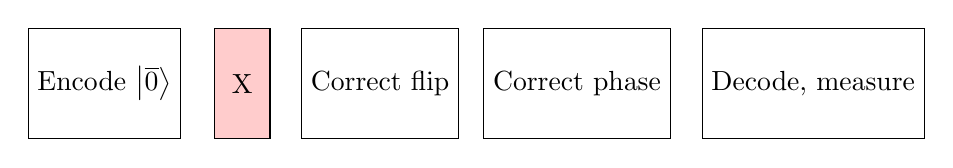
\begin{tikzpicture}
    \node[block] (init) at (0, 0) {Encode $\ket{\overline{0}}$};
    \node[redblock] (xgate) at (1.75, 0) {X};
    \node[block] (cf) at (3.5, 0) {Correct flip};
    \node[block] (cp) at (6, 0) {Correct phase};
    \node[block] (end) at (9, 0) {Decode, measure};
  \end{tikzpicture}
  \begin{center}
    \includegraphics[width=8cm]{noisefree_corr}
  \end{center}
\end{frame}

\begin{frame}{7-qubit code: Fidelity of X Gate under \textcolor{red!20}{Depolarization}}
  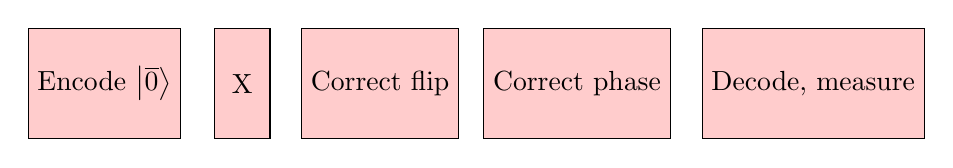
\begin{tikzpicture}
    \node[redblock] (init) at (0, 0) {Encode $\ket{\overline{0}}$};
    \node[redblock] (xgate) at (1.75, 0) {X};
    \node[redblock] (cf) at (3.5, 0) {Correct flip};
    \node[redblock] (cp) at (6, 0) {Correct phase};
    \node[redblock] (end) at (9, 0) {Decode, measure};
  \end{tikzpicture}
  \begin{center}
    \includegraphics[width=8cm]{noisy_corr}
  \end{center}
\end{frame}

\begin{frame}{7-qubit code: Simulation vs running on quantum computers?}
    - The states should be clearly defined, but noise dominates the system
    \begin{center}
        \includegraphics[width=8cm]{7-melbourne-fidelity}
    \end{center}
\end{frame}

\begin{frame}{7-qubit code: Useful with lower error probability}
  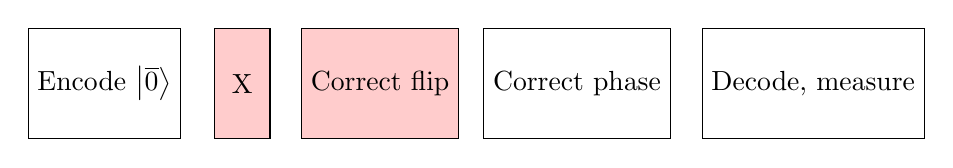
\begin{tikzpicture}
    \node[block] (init) at (0, 0) {Encode $\ket{\overline{0}}$};
    \node[redblock] (xgate) at (1.75, 0) {X};
    \node[redblock] (cf) at (3.5, 0) {Correct flip};
    \node[block] (cp) at (6, 0) {Correct phase};
    \node[block] (end) at (9, 0) {Decode, measure};
  \end{tikzpicture}
  \includegraphics[width=\textwidth]{7-steane-comparison}
\end{frame}

\begin{frame}{7-qubit code: Adding Error Correction at different Timesteps}
  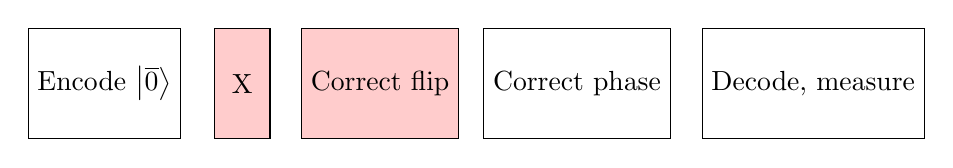
\begin{tikzpicture}
    \node[block] (init) at (0, 0) {Encode $\ket{\overline{0}}$};
    \node[redblock] (xgate) at (1.75, 0) {X};
    \node[redblock] (cf) at (3.5, 0) {Correct flip};
    \node[block] (cp) at (6, 0) {Correct phase};
    \node[block] (end) at (9, 0) {Decode, measure};
  \end{tikzpicture}
  \includegraphics[width=\textwidth]{7-schedule-comparison}
\end{frame}

\end{document}
